\documentclass{beamer}
\usetheme{CambridgeUS}
\usepackage[spanish]{babel}
\usepackage[utf8]{inputenc}
\usefonttheme{professionalfonts}
\usepackage{times}
\usepackage{tikz}
\usepackage{amsmath}
\usepackage{mathrsfs}       %negrita en ecuaciones
\usepackage{upgreek}        %negrita en letras griegas
\usepackage{mhchem}         %para reacciones químicas
\usepackage{url}
\usepackage{verbatim}
\usetikzlibrary{arrows,shapes}
\usepackage{graphicx}
\usepackage{subfigure}
\graphicspath{{imagenes/}}

%bibliografia
\usepackage[backend=bibtex,style=numeric]{biblatex}
\bibliography{dddddd.bib}
%\addbibresource{dddddd.bib}  

\author{Daniel Villarreal}
\title{Sustentación de Trabajo de Grado}

%funciones creadas
\newcommand{\negd}[1]{\mathbf{#1}}    %negrita letras normales
\newcommand{\neggr}[1]{\boldsymbol{#1}}

\begin{document}

%página 1
\begin{frame}
     \frametitle{Estimación de la Irradiancia Solar en la República de Panamá}
     %\framesubtitle{Asesor: Dr. Abdoulaye Diallo, Estudiante: Daniel Villarreal}
      \begin{figure}[h!]
         \centering \subfigure{
\includegraphics[width=2cm, height=2cm]{logo_utp}}
         \hspace{5cm}
         \centering \subfigure{
\includegraphics[width=3cm, height=1cm]{senacyt}}
      \end{figure}
      \begin{center}
         {\scshape \scriptsize Universidad Tecnológica de Panamá \par}
         {\scshape \scriptsize Facultad de Ciencias y Tecnología \par}
         {\scshape \scriptsize Maestría en Ciencias Físicas \par}
         \vspace{0.3cm}
         \scriptsize Presentado por: \\
         \scriptsize Daniel Villarreal Chiari \\
         \begin{large}
            \scriptsize Asesor: \\
            \scriptsize Abdoulaye F. Diallo \\
         \end{large}
      \end{center}
\vfill
Panamá, Ciudad de Panamá, \hfill Octubre 2018
\end{frame}

%página 2
\begin{frame}[t,allowframebreaks]
    \frametitle{Contenido}
    \tableofcontents
\end{frame}

%página 3
\section{La Radiación Solar}
\begin{frame}
   \frametitle{La Radiación Solar}
   \begin{figure}[h!]
   \begin{minipage}{0.4\textwidth}
   \begin{flushleft}
   \begin{itemize}
      \item\scriptsize En el Sol, ocurren reacciones nucleares, que dependen de sus características estructurales \cite{duffie2013solar}.
      \item\scriptsize Los fotones resultantes de estas reacciones nucleares transportan la energía producida \cite{fisicasol}. 
      \item\scriptsize Las radiación visible e infraroja son las que en mayor cantidad atraviesan la atmósfera terrestre \cite{duffie2013solar}. 
   \end{itemize}
   \end{flushleft} 
   \end{minipage}
   \begin{minipage}{0.5\textwidth}
      \centering 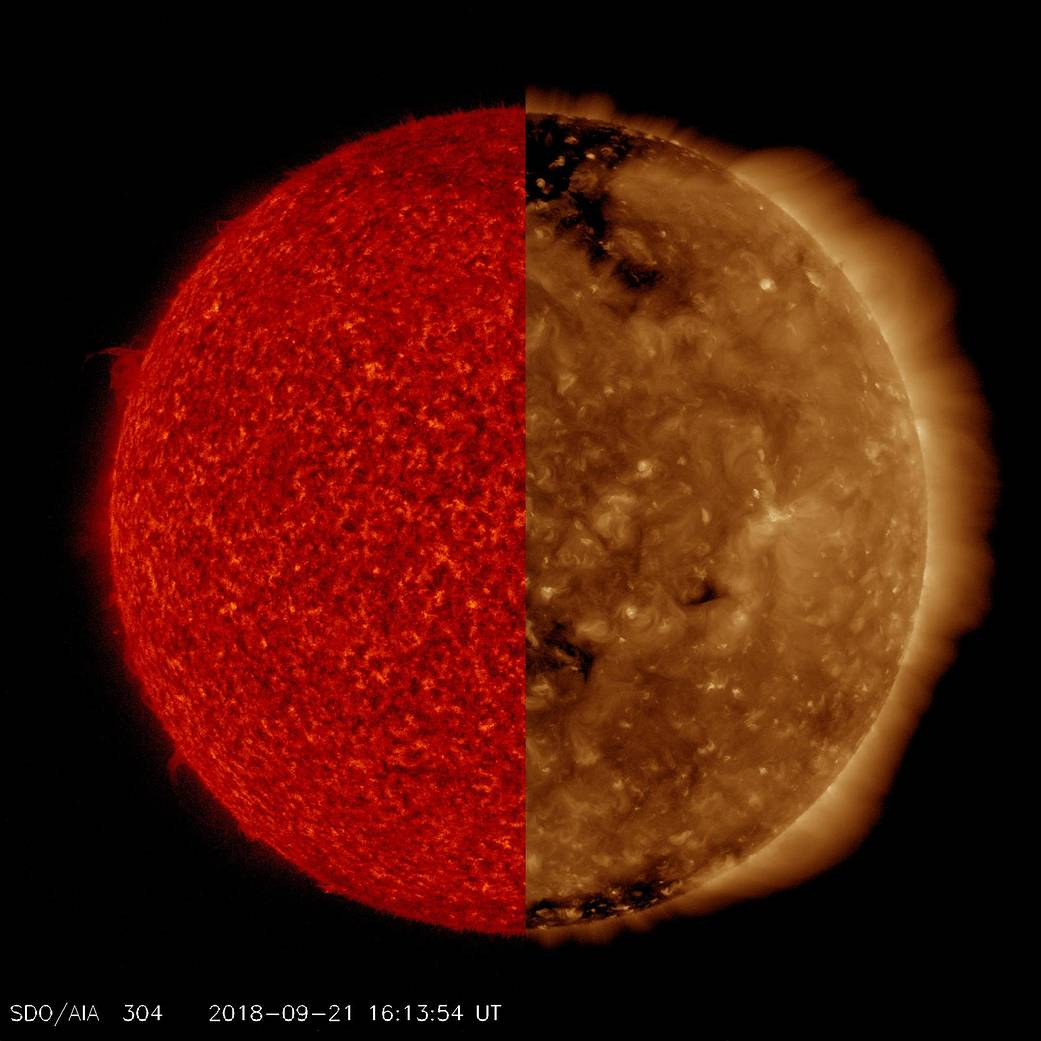
\includegraphics[width=4.5cm, height=4.5cm]{radiacion_solar}
      \caption{\tiny Imagen del Sol en ultravioleta (izq.) e infrarojo (der.). Fuente: \path{NASA/GSFC/Solar_Dynamics_Observatory}}
   \end{minipage}
   \end{figure}
\end{frame}

%página 4
\subsection{El Sol}
\begin{frame}
  \frametitle{El Sol}
  \begin{figure}[h!]
  \begin{minipage}{0.4\textwidth}
  \begin{flushleft}

  \begin{itemize}
      \item\scriptsize Es una estrella que se encuentra en promedio a una distancia de $1,5 \times 10^{11} m$ de la Tierra (una unidad astronómica 1 UA).
      \item\scriptsize Se encuentra en etapa de secuencia principal.
      \item\scriptsize Su fuente de energía es la cadena protón-protón
  \end{itemize}
  \end{flushleft}
  \end{minipage}
  \hspace{1cm}
  \begin{minipage}{0.4\textwidth}
     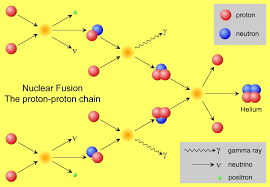
\includegraphics[width=5.5cm, height=4.5cm]{cadena_pp}
     \caption{\tiny Cadena PP. Fuente: \path{ciencias.bogota.unal.edu.co}}
  \end{minipage}
  \end{figure}
  \begin{equation} 4\; \ce{^{1}H} \to \ce{^{4}He} + 2 e^{+} + 2 \nu + 2 \gamma + 24.16 MeV \end{equation}
\end{frame}


%paǵina 5
\subsection{Definiciones}
\begin{frame}
   \frametitle{Definiciones}
   \begin{itemize}
      \item Irradiancia Solar
      \item Radiación Solar Directa
      \item Radiación Difusa
      \item Radiación Solar Reflejada
      \item Radiación Solar Global
   \end{itemize}
\end{frame}

%página 6
\begin{frame}
   \frametitle{Hora Sol Pico y Constante Solar}
   \framesubtitle{Dos Definiciones Importantes}
   \begin{figure}
      \begin{minipage}{0.4\textwidth}
         \textbf{Hora Sol Pico}(hsp) \par
         \vspace{0.5 cm}
         \scriptsize Considera el caso hipotético de una irradiancia constante de $1000 \; W/m^2$ , durante un tiempo relativamente corto, de modo 
         que la energía incidente sea igual a la energía diaria total \cite{hora_sol_pico}.\par 
         \centering 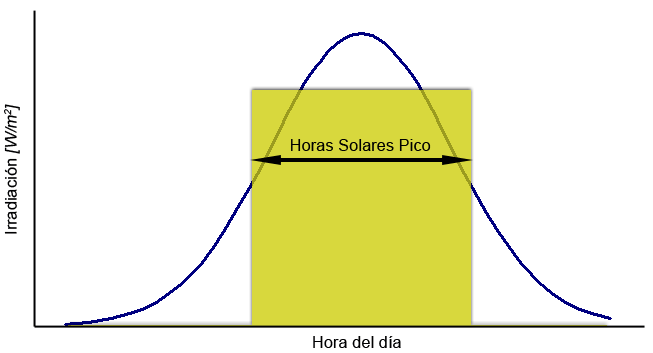
\includegraphics[width=4.5cm, height=3.5cm]{hora_sol_pico}
         \caption{\tiny Hora Sol Pico. Fuente: \path{es.wikipedia.org/wiki/Hora_solar_pico}}
      \end{minipage}
      \hspace{0.5cm} 
      \begin{minipage}{0.4\textwidth}
         \textbf{Constante Solar} \par
         \vspace{0.5 cm}
         \scriptsize Potencia lumínica por unidad de área recibida en una superficie perpendicular a la dirección de propagación de la radiación a la
         distancia Sol-Tierra promedio en las capas externas de la atmósfera se denomina Constante Solar (Gsc) \cite{johnson1954solar}. \par
         En este trabajo se utiliza el valor de constante solar adoptado por el  Centro Mundial de Radiación (World Radiation Center WRC):  
         $$1367 \; \frac{W}{m^2}$$
      \end{minipage}
   \end{figure}
\end{frame}

%página 7
\subsection{Radiación Solar Extraterrestre}
\begin{frame}
   \frametitle{Radiación Solar Extraterrestre}
   Para estimar la irradiancia solar extraterrestre, en 1983, Iqbal utiliza el modelo de
   Spencer (1971), en la forma de la ecuación \ref{iqbal}
   \begin{equation}
      \label{iqbal}
      G_{on} = \begin{cases}
           G_{sc}(1.000110 + 0.034221 \cos B + 0.001280\sin B +
                    \\ 0.000719 \cos 2B + 0.000077 \sin 2B)\\
           \\
           \boxed{B = (n - 1) \frac{360}{365}}\end{cases}
   \end{equation}
\end{frame}

%página 8
\begin{frame}
   \frametitle{Ángulo de Incidencia de la Radiación Solar}
   \scriptsize La relación geométrica entre un plano orientado en una dirección arbitraria relativa
   a la Tierra, y la radiación solar incidente, puede ser descrita en función de ángulos
   relativos a la posición del Sol. \par
   Estos ángulos son:\par
   \begin{figure}
   \begin{minipage}{0.5\textwidth} 
   \begin{itemize}
      \item \textbf{Ángulo de Acimut de la Superficie} $\gamma$, 
      \item \textbf{Latitud} $\phi$,
      \item \textbf{Inclinación de la Superficie} $\beta$,
      \item \textbf{Ángulo Horario} $\omega$,
   \end{itemize}
   \end{minipage}
   \begin{minipage}{0.4\textwidth}
      \begin{itemize}
         \item \textbf{Declinación} $\delta$,
         \item \textbf{Ángulo de Incidencia} $\theta$,
         \item \textbf{Ángulo de Elevación del Sol} $e$,
         \item \textbf{Acimut del Sol} $\gamma_s$,
      \end{itemize}
   \end{minipage}
   \end{figure}

   \begin{align}
     \notag
     \label{incidencia}
     \cos\theta = & \; \sin\delta (\sin\phi \cos\beta - \cos\phi \sin\beta \cos\gamma) \; + \; \\
     & \; \cos\delta(\cos\phi \cos\beta \cos\omega + \sin\phi \sin\beta \cos\gamma
       \cos\omega + \sin\beta \sin\gamma \sin\omega)
   \end{align} 
   Para el caso de una superficie horizontal el ángulo de inclinación y la orientación acimutal es cero; por lo
   que bajo estas condiciones (\ref{incidencia}) se reduce a la expresión (\ref{inc_hor}).
   \begin{equation}
     \label{inc_hor}
     \cos\theta = \; \sin\delta\sin\phi \; + \; \cos\delta\cos\phi\cos\omega
   \end{equation}   
\end{frame}

%página 9
\begin{frame}
   \frametitle{Radiación Solar Promedio Diaria Incidente en una Superficie Horizontal}
   \scriptsize La irradiancia solar instántanea $G_o \;$ se define como:
   \begin{equation}
     \label{irradiancia}
      G_o = G_{on} \cos\theta
   \end{equation}
   en donde, $G_{on}$ está dada por la relación (\ref{iqbal}) y $\theta$ el ángulo de incidencia de la radiación solar directa sobre la superficie.
   Sustituyendo (\ref{inc_hor}) y (\ref{iqbal}) en (\ref{irradiancia}), se obtiene:
   \begin{align}
      \notag
      \label{irradiancia_2}
      G_o = & \; G_{sc} (1.000110 \; + \; 0.034221 \cos B \; + \; 0.001280\sin B \; + \; 0.000719 \cos 2B \; \\
            & \; \; \; \; \; \; + \; 0.000077 \sin 2B)(\sin\delta\sin\phi \; + \; \cos\delta\cos\phi\cos\omega)
   \end{align}
   Integrando (\ref{irradiancia_2}) desde el amenecer hasta el atardecer, se obtiene la radiación solar directa que se recibe en una superficie horizontal a lo
   largo del día:
   \begin{equation} \label{energia_diaria} H_o = \; G_{on} \big(\cos\phi\cos\delta\sin\omega_s \; + \; \frac{\pi\omega_s}{180}\sin\phi\sin\delta \big) \end{equation}
   donde $H_o$ es la energía diaria sobre una superficie horizontal, $G_{on}$ es la irradiancia estimada por el modelo de Iqbal (ecuación (\ref{iqbal})).\par

   La ecuación (\ref{energia_diaria}) es el modelo que se usa en este trabajo para estimar la radiación solar directa que incide sobre una superficie horizontal.
\end{frame}

%página 10
\subsection{Influencia de la Atmósfera en la Radiación Solar}
\begin{frame}
   \frametitle{Influencia de la Atmósfera en la Radiación Solar}
   \framesubtitle{Dispersión, Absorción y Reflexión}
   \begin{figure}
      \begin{minipage}{0.4\textwidth}
         \scriptsize
         La atmósfera terrestre modifica la radiación solar que se transmite através de ella. Esta modificación sucede mediante los fenómenos de \textbf{dispersión, absorción
         y reflexión}. Cada fenómeno depende de la longitud de onda de la radiación solar y de las dimensiones de las partículas atmosféricas que interactúan. Por
         lo que estas suceden en diferentes secciones de la atmósfera. Esto debido a que las partículas más grandes se encuentran en las capas más bajas y las partículas
         más pequeñas en las capas superiores \cite{scatter,spectral_rad}.
      \end{minipage}
      \hspace{0.7cm}
      \begin{minipage}{0.5\textwidth}
         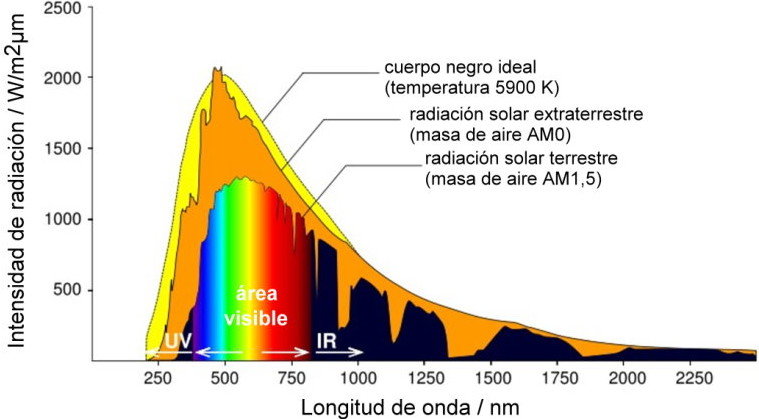
\includegraphics[height=3.5cm,width=5.0cm]{atmosfera}
         \caption{\tiny Espectro de Irradiancia Solar, Fuente: \path{http://klimat.czn.uj.edu.pl/}}
      \end{minipage}
    \end{figure}
\end{frame}

%página 11
\subsection{Modelos de Radiación Solar Diaria}
\begin{frame}
   \scriptsize
   A partir de la ecuación (\ref{energia_diaria}) se puede estimar la energía diaria en las capas externas de la atmósfera. Pero la radiación solar
   se ve afectada por la interacción con la atmósfera. Por lo tanto, para predecir la radiación solar que se recibe en la superficie terrestre, es necesario
   emplear otras herramientas. Estás herramientas son de dos tipos: la primera que busca predicciones de datos en tiempo real y la otra hace estimaciones
   en base a datos históricos. Para utilizar herramientas del segundo tipo se necesita la construcción de series temporales de la radiación solar histórica \cite{predicc_solar}. \par

   Uno de los métodos más usados para análisis de series de tiempo son los llamados procesos autoregresivos, en particular: ARMA y ARIMA. En este trabajo se utiliza el proceso ARMA porque la radiación solar histórica 
   medida no muestra patrones de ascendencia o descendencia constante, lo cual permite el uso de un proceso ARMA.  
\end{frame}

%páǵina 12
\subsection{Procesos Autoregresivos de Media Móvil (ARMA)}
\begin{frame}
   \frametitle{Procesos Autoregresivos de Media Móvil (ARMA)}
   \scriptsize
   \begin{itemize}
      \item En ocasiones es posible modelar una variable en función de sus valores pasados. 
      \vspace{1cm}
      \item Esta es la principal idea que da origen a los polinomios autoregresivos y de media móvil.
      \vspace{1cm}
      \item La combinación de ambos tipos produce una serie autoregresiva de media móvil.
      \vspace{1cm}
      \item Este tipo de series se conoce con el nombre de \textit{series temporales}.
   \end{itemize}
\end{frame}

%página 13
\begin{frame}
   \frametitle{Series Temporales}
   \scriptsize
   Una serie temporal es una sucesión de valores de una variable observada en determinados instantes de tiempo. El análisis de series temporales se basa
   principalmente en: la tendencia, estacionalidad, variación cíclica y/o variaciones accidentales de la misma \cite{ser_temp_1,ser_tmp_2}.
   \vspace{0.1cm}
   \begin{itemize}
      \item Los modelos que se producen a partir del análisis de series temporales pueden ser series univariantes o multivariantes.
      \item Una serie temporal es una secuencia aleatoria de variables ordenadas en el tiempo (un proceso estocástico), lo cual se puede representar como:
            \begin{equation}
              \label{serie_temporal}
              Y_t(\eta), \;\; t = \mbox{...}, t-2, t-1, t, t + 1, t + 2, \mbox{...}
            \end{equation}
            donde t es el instante en que se realiza la observación $Y_t(\eta)$.
   \end{itemize}
   \begin{figure}[h!]
      \centering 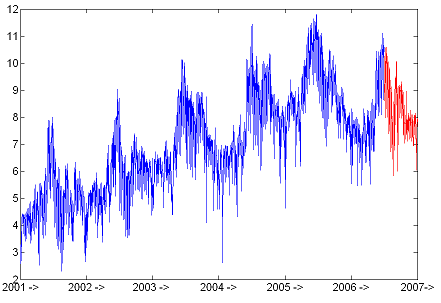
\includegraphics[heigth=4.1cm,width=4.5cm]{serie_de_tiempo}
      \caption{\tiny Ejemplo de Serie de Tiempo. Fuente: \path{https://www.ugr.es/~jherrera/resultados.html}}
   \end{figure}
\end{frame}

%página 14
\begin{frame}
   \frametitle{Series Temporales: Procesos Estocásticos}
   \begin{itemize}
   \scriptsize
   \item  Una serie temporal, es una secuencia aleatoria de variables ordenadas en el tiempo. Es por esto que las series temporales son
   consideradas un tipo de proceso estocástico en el cual las variables están relacionadas por el tiempo.
   \begin{equation} \label{serie_temporal}
      Y_t(\eta), \;\; t = \mbox{...}, t-2, t-1, t, t + 1, t + 2, \mbox{...}
   \end{equation}
    donde t es el instante en que se realiza la observación $Y_t(\eta)$
   \item Los procesos estocásticos se suelen determinar en términos de la función de distribución asociada al proceso. Sin embargo, obtener la función de distribución
   es complejo; por lo que se usan los dos primeros momentos \cite{ser_temp_3}.
   \item El primer momento corresponde al conjunto de las medias de todas las variables aleatorias del proceso.
        \begin{equation}
        E(Y_t) = \mu_t < \infty, \;\; t=0,\pm1,\pm2,...,
        \end{equation}

        en donde, $\mu_t$ es la media del proceso en el instante $t$.
   \item El segundo momento corresponde al conjunto

    
   \end{itemize}
\end{frame}

%bibliografia
\begin{frame}[t,allowframebreaks]
   \frametitle{Referencias}
   \printbibliography
\end{frame}

\end{document}
